\appendix

\section{Appendix}\label{app}

To provide empirical context for our literature review, we implemented a multi-agent coordination experiment using Proximal Policy Optimization (PPO) in two environments from the Multi-Agent Particle Environment (MPE) suite: Simple Spread (cooperation) and Simple Adversary (competition). These environments require multiple agents to coordinate their movements to cover distinct landmarks without collisions, while escaping from the adversary agent. These games represent a fundamental resource allocation challenge where spatial positions serve as contested resources.

\subsection{Simple Spread Environment}

The Simple Spread environment instantiates key challenges in competitive multi-agent learning. Three agents must simultaneously learn to occupy different landmarks while avoiding collisions with each other. Each agent observes its own position, velocity, and relative positions to landmarks and other agents. The reward structure encourages agents to cover landmarks while penalizing collisions, creating an implicit resource competition where optimal positioning requires coordination rather than pure competition.

\subsection{Simple Adversary Environment}

The Simple Adversary environment blends cooperation and competition by pitting two “good” agents (blue) against one adversary (red), with landmarks equal to the number of good agents. Each episode, only the good agents know which landmark is the target. They are rewarded for proximity to the target, while the adversary—unaware of the target’s identity—must infer it from the good agents’ behavior and is rewarded for approaching it. This setup forces good agents to coordinate and deceive, while the adversary predicts and intercepts. With observations including relative positions and discrete movement actions, the environment serves as a concise testbed for partial observability, deception, and adaptive opponent modeling in competitive multi-agent reinforcement learning.

These tasks exemplify the core challenges addressed in our literature review: agents must solve credit assignment problems (determining which agent should target which landmark), handle non-stationarity (as other agents' policies evolve during training), and develop coordination strategies that emerge from individual learning processes.


\subsection{PPO Implementation}

Our implementation follows the centralized training with decentralized execution paradigm, where agents share a critic network during training but execute policies independently. We track key metrics including episode rewards, episode lengths, value function losses, and policy gradient losses to analyze learning dynamics and convergence properties.

The experiment demonstrates empirically how multi-agent environments create natural curricula—as agents improve, the coordination challenge increases correspondingly. This observation directly motivates the theoretical frameworks examined in our literature review, particularly regarding emergent complexity in competitive resource environments and the challenges of achieving stable learning in non-stationary multi-agent settings.

\subsection{Neural Network Architecture}

\subsubsection{Policy Network Architecture}

\begin{verbatim}
policy_kwargs = dict(
    net_arch=[256, 256, 128],
    activation_fn=torch.nn.Tanh)
\end{verbatim}

\textbf{Architecture Description:}
\begin{itemize}
    \item \textbf{Input Layer}: Flattened observation vectors from the environment (agent positions, velocities, relative distances)
    \item \textbf{Hidden Layer 1}: 256 neurons with Tanh activation
    \item \textbf{Hidden Layer 2}: 256 neurons with Tanh activation
    \item \textbf{Hidden Layer 3}: 128 neurons with Tanh activation
    \item \textbf{Output Layers}:
    \begin{itemize}
        \item \textbf{Actor head}: Continuous action outputs (movement forces in x, y directions)
        \item \textbf{Critic head}: Single value estimate for state evaluation
    \end{itemize}
\end{itemize}

\subsubsection{Activation Function Choice}
\begin{itemize}
    \item \textbf{Tanh activation}: Chosen for continuous control tasks as it provides bounded outputs ($-1, 1$), naturally suited for movement commands in the adversarial environment
    \item \textbf{Smooth gradients}: Facilitates stable learning in competitive multi-agent settings
\end{itemize}

\subsection{Training Methodology}

\subsubsection{Algorithm: Proximal Policy Optimization (PPO)}

\begin{verbatim}
model = PPO(
    ActorCriticPolicy,
    env=env,
    learning_rate=3e-4,
    n_steps=256,
    batch_size=512,
    ent_coef=0.01,
    gamma=0.98,
    gae_lambda=0.95,
    verbose=1,
    tensorboard_log="./ppo_marl_tb/",
    policy_kwargs=policy_kwargs)
\end{verbatim}

\subsubsection{Hyperparameter Configuration}

\textbf{Learning Parameters:}
\begin{itemize}
    \item \textbf{Learning Rate}: 3e-4 (conservative rate for stable competitive learning)
    \item \textbf{Rollout Buffer}: 256 steps per update cycle
    \item \textbf{Batch Size}: 512 (large batches for reduced variance in competitive settings)
\end{itemize}

\textbf{PPO-Specific Parameters:}
\begin{itemize}
    \item \textbf{Entropy Coefficient}: 0.01 (encourages exploration while maintaining policy stability)
    \item \textbf{Discount Factor ($\gamma$)}: 0.98 (values future rewards highly for strategic planning)
    \item \textbf{GAE Lambda}: 0.95 (Generalized Advantage Estimation for bias-variance trade-off)
\end{itemize}

\subsubsection{Training Scale}
\begin{itemize}
    \item \textbf{Total Timesteps}: 500,000 (extended training for complex strategy development)
    \item \textbf{Training Updates}: $\sim$1,953 PPO updates (500,000 $\div$ 256 rollout buffer)
    \item \textbf{Episode Length}: Maximum 100 steps per episode
\end{itemize}

\subsection{Multi-Agent Training Approach}

\subsubsection{Parameter Sharing Strategy}
\begin{itemize}
    \item \textbf{Centralized Training}: All agents (both good agents and adversaries) share the same policy network parameters
    \item \textbf{Decentralized Execution}: During evaluation, each agent acts independently based on local observations
    \item \textbf{Homogeneous Agents}: Identical network architecture for all agent types, with role differentiation emerging through reward structure
\end{itemize}

\subsubsection{Environment Preprocessing Pipeline}

\begin{verbatim}
env = ss.black_death_v3(env)               # Handle agent termination
env = ss.pad_observations_v0(env)          # Standardize obs dimensions
env = ss.flatten_v0(env)                   # Convert to vector format
env = aec_to_parallel(env)                 # Enable simultaneous actions
env = ss.pettingzoo_env_to_vec_env_v1(env) # Vectorization compatibility
\end{verbatim}

\subsubsection{Observation Processing}
\begin{itemize}
    \item \textbf{Input}: Multi-dimensional observations including agent positions, velocities, and relative distances
    \item \textbf{Flattening}: Converts structured observations to flat vectors suitable for MLP processing
    \item \textbf{Padding}: Ensures consistent input dimensions across different agent types
    \item \textbf{Normalization}: Handled implicitly through environment wrappers
\end{itemize}

\subsubsection{Competitive Learning Dynamics}
\begin{itemize}
    \item \textbf{Zero-Sum Structure}: Good agents maximize rewards for reaching landmarks while avoiding capture; adversaries maximize rewards for catching good agents
    \item \textbf{Self-Play Training}: Agents improve by competing against increasingly sophisticated opponents
    \item \textbf{Emergent Complexity}: Strategic behaviors emerge through competitive pressure rather than explicit programming
    \item \textbf{Natural Curriculum}: Difficulty scales automatically as agents improve
\end{itemize}

\subsubsection{Training Stability Considerations}
\begin{itemize}
    \item \textbf{Conservative Hyperparameters}: Lower learning rates and entropy coefficients prevent instability in non-stationary multi-agent environments
    \item \textbf{Large Batch Sizes}: Reduce variance in gradient estimates when multiple agents are learning simultaneously
    \item \textbf{Extended Training}: 500,000 timesteps allow for sophisticated strategy development and convergence
\end{itemize}

\noindent
This architecture and training methodology enables the emergence of complex competitive behaviors such as coordinated pursuit strategies, evasion patterns, and spatial awareness through pure reinforcement learning optimization.

\subsection{Connection to Literature Review}

This practical implementation grounds our literature review in concrete multi-agent learning challenges by leveraging both the Simple Spread and Simple Adversary environments. The Simple Spread task encapsulates fundamental themes from the literature, such as resource competition for spatial positions, coordination under partial observability, and the emergence of complex group behaviors from simple, decentralized policies. In contrast, the Simple Adversary environment introduces an explicit adversarial element, requiring agents to balance cooperation with deception and opponent modeling as they navigate a setting where one agent seeks to thwart the goals of the others. The empirical training dynamics observed in our experiments—including convergence patterns, the development of coordinated strategies, and adaptive responses to adversarial pressure—provide a tangible context for understanding the theoretical contributions and algorithmic advances discussed in the literature review. By examining both cooperative and mixed-motive scenarios, our implementation illustrates how diverse multi-agent environments instantiate and challenge the core ideas explored in contemporary research.

The experiment's training results (\figureref{fig:training_history},  \figureref{fig:training_dashboard} and \figureref{fig:adversary}) illustrate the learning curves and coordination development that motivate the need for sophisticated multi-agent algorithms, directly connecting our practical experience to the surveyed theoretical advances in competitive multi-agent reinforcement learning.

\begin{figure}[htpb]
    \centering
    \includesvg[width=0.9\textwidth]{latex/imgs/training_history.svg}
    \caption{PPO training metrics on Simple Spread environment. Clockwise from top-left: episode rewards, episode lengths, policy losses, and value function losses over 30k timesteps.}
    \label{fig:training_history}
\end{figure}

\begin{figure}[htpb]
    \centering
    \includesvg[width=0.9\textwidth]{latex/imgs/dashboard.svg}
    \caption{Multi-agent coordination dashboard. Clockwise from top-left: showing reward progression, agent behaviors, value loss, and coordination score during PPO training.}
    \label{fig:training_dashboard}
\end{figure}

\begin{figure}[htpb]
    \centering
    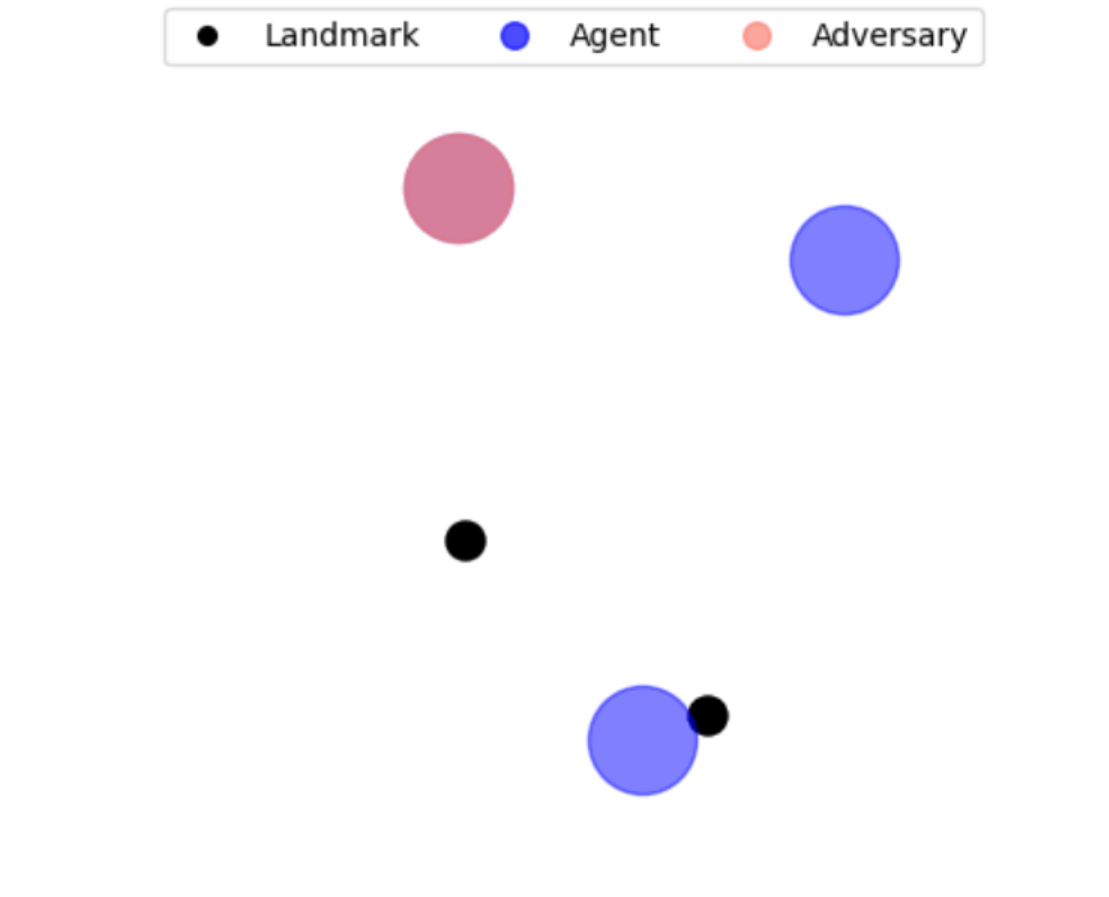
\includegraphics[width=0.75\linewidth]{latex/imgs/adversary_anim.png}
    \caption{Screenshot from Simple Adversary training process. The blue "good" agents have to reach a landmark and escape the red adversary.}
    \label{fig:adversary}
\end{figure}
